\documentclass{beamer}
\usepackage[utf8]{inputenc}

\usetheme{Madrid}
\usecolortheme{default}
\usepackage{amsmath,amssymb,amsfonts,amsthm}
\usepackage{txfonts}
\usepackage{tkz-euclide}
\usepackage{listings}
\usepackage{adjustbox}
\usepackage{array}
\usepackage{tabularx}
\usepackage{gvv}
\usepackage{lmodern}
\usepackage{circuitikz}
\usepackage{tikz}
\usepackage{graphicx}
\usepackage[T1]{fontenc}
\usepackage[utf8]{inputenc}

\lstset{
  language=Python,
  basicstyle=\ttfamily\small,
  breaklines=true,
  literate={λ}{{$\lambda$}}1
}



\setbeamertemplate{page number in head/foot}[totalframenumber]

\usepackage{tcolorbox}
\tcbuselibrary{minted,breakable,xparse,skins}



\definecolor{bg}{gray}{0.95}
\DeclareTCBListing{mintedbox}{O{}m!O{}}{%
  breakable=true,
  listing engine=minted,
  listing only,
  minted language=#2,
  minted style=default,
  minted options={%
    linenos,
    gobble=0,
    breaklines=true,
    breakafter=,,
    fontsize=\small,
    numbersep=8pt,
    #1},
  boxsep=0pt,
  left skip=0pt,
  right skip=0pt,
  left=25pt,
  right=0pt,
  top=3pt,
  bottom=3pt,
  arc=5pt,
  leftrule=0pt,
  rightrule=0pt,
  bottomrule=2pt,
  toprule=2pt,
  colback=bg,
  colframe=orange!70,
  enhanced,
  overlay={%
    \begin{tcbclipinterior}
    \fill[orange!20!white] (frame.south west) rectangle ([xshift=20pt]frame.north west);
    \end{tcbclipinterior}},
  #3,
}
\lstset{
    language=C,
    basicstyle=\ttfamily\small,
    keywordstyle=\color{blue},
    stringstyle=\color{orange},
    commentstyle=\color{green!60!black},
    numbers=left,
    numberstyle=\tiny\color{gray},
    breaklines=true,
    showstringspaces=false,
}
\begin{document}

\title 
{5.2.18}
\date{September 14,2025}


\author 
{Bhoomika V - EE25BTECH11015}




\frame{\titlepage}
\begin{frame}{Question}
Solve the following system of linear equation.\\ 
$8x + 5y = 9$\\ 
$3x + 2y = 4$\\ \\ 
\end{frame}

\begin{frame}{Solution}
We are solving the system:
\[
8x + 5y = 9, \quad 3x + 2y = 4
\]

Coefficient matrix and vector
\[
A = \begin{bmatrix} 8 & 5 \\ 3 & 2 \end{bmatrix}, \quad 
b = \begin{bmatrix} 9 \\ 4 \end{bmatrix}
\]
\end{frame}

\begin{frame}{Solution}
Performing row operations (RREF)

\(R_1 \to \frac{R_1}{8}\)
\[
\begin{bmatrix} 8 & 5 \\ 3 & 2 \end{bmatrix} 
\;\overset{R_1 \to R_1/8}{\longrightarrow}\;
\begin{bmatrix} 1 & 5/8 \\ 3 & 2 \end{bmatrix}, \quad
b = \begin{bmatrix} 9 \\ 4 \end{bmatrix} 
\;\overset{R_1 \to R_1/8}{\longrightarrow}\;
\begin{bmatrix} 9/8 \\ 4 \end{bmatrix}
\]
\end{frame}

\begin{frame}{Solution}
Eliminate first column in \(R_2\): \(R_2 \to R_2 - 3R_1\)
\[
\begin{bmatrix} 1 & 5/8 \\ 3 & 2 \end{bmatrix} 
\;\overset{R_2 \to R_2 - 3R_1}{\longrightarrow}\;
\begin{bmatrix} 1 & 5/8 \\ 0 & 1/8 \end{bmatrix}, \quad
b = \begin{bmatrix} 9/8 \\ 4 \end{bmatrix} 
\;\overset{R_2 \to R_2 - 3R_1}{\longrightarrow}\;
\begin{bmatrix} 9/8 \\ 5/8 \end{bmatrix}
\]

\(R_2 \to 8R_2\)
\[
\begin{bmatrix} 1 & 5/8 \\ 0 & 1/8 \end{bmatrix} 
\;\overset{R_2 \to 8R_2}{\longrightarrow}\;
\begin{bmatrix} 1 & 5/8 \\ 0 & 1 \end{bmatrix}, \quad
b = \begin{bmatrix} 9/8 \\ 5/8 \end{bmatrix} 
\;\overset{R_2 \to 8R_2}{\longrightarrow}\;
\begin{bmatrix} 9/8 \\ 5 \end{bmatrix}
\]
\end{frame}

\begin{frame}{Solution}
Eliminate second column in \(R_1\): \(R_1 \to R_1 - (5/8)R_2\)
\[
\begin{bmatrix} 1 & 5/8 \\ 0 & 1 \end{bmatrix} 
\;\overset{R_1 \to R_1 - (5/8)R_2}{\longrightarrow}\;
\begin{bmatrix} 1 & 0 \\ 0 & 1 \end{bmatrix}, \quad
b = \begin{bmatrix} 9/8 \\ 5 \end{bmatrix} 
\;\overset{R_1 \to R_1 - (5/8)R_2}{\longrightarrow}\;
\begin{bmatrix} -1 \\ 5 \end{bmatrix}
\]

 Answer 
\[
x = -1, \quad y = 5
\]
\end{frame}

\begin{frame}[fragile]
    \begin{lstlisting}
 // linear.c
#include <stdio.h>

// Function to solve system of 2 equations:
// a1*x + b1*y = c1
// a2*x + b2*y = c2
// Returns solution in x_out and y_out
void solve_linear(float a1, float b1, float c1,
                  float a2, float b2, float c2,
                  float *x_out, float *y_out) {
    float det = a1*b2 - a2*b1;
    if (det == 0) {
        *x_out = 0;
        *y_out = 0;
        return;
    }
    *x_out = (c1*b2 - c2*b1) / det;
    *y_out = (a1*c2 - a2*c1) / det;
}
     \end{lstlisting}
\end{frame}

\begin{frame}[fragile]
    \frametitle{Python Code}
    \begin{lstlisting}
import numpy as np
import matplotlib.pyplot as plt
import ctypes
import os

# --- Load the C library ---
try:
    c_lib = ctypes.CDLL('./linear.so')  # use linear.dll on Windows
except OSError:
    print("Error: 'linear.so' not found. Compile using: gcc -shared -o linear.so -fPIC linear.c")
    exit()
    \end{lstlisting}
\end{frame}

\begin{frame}[fragile]
    \frametitle{Python Code}
    \begin{lstlisting}
# Define argument and return types
c_lib.solve_linear.argtypes = [ctypes.c_float, ctypes.c_float, ctypes.c_float,
                               ctypes.c_float, ctypes.c_float, ctypes.c_float,
                               ctypes.POINTER(ctypes.c_float),
                               ctypes.POINTER(ctypes.c_float)]
c_lib.solve_linear.restype = None

# --- Coefficients of system ---
# 8x + 5y = 9
# 3x + 2y = 4
a1, b1, c1 = 8.0, 5.0, 9.0
a2, b2, c2 = 3.0, 2.0, 4.0
    \end{lstlisting}
\end{frame}

\begin{frame}[fragile]
    \frametitle{Python Code}
    \begin{lstlisting}
# Allocate memory for outputs
x_out = ctypes.c_float()
y_out = ctypes.c_float()

# Call C function
c_lib.solve_linear(a1, b1, c1,
                   a2, b2, c2,
                   ctypes.byref(x_out),
                   ctypes.byref(y_out))

x_sol, y_sol = x_out.value, y_out.value
print(f"Solution: x = {x_sol:.2f}, y = {y_sol:.2f}")

# --- Plotting ---
x = np.linspace(-5, 5, 400)
y1 = (c1 - a1*x)/b1   # from 8x + 5y = 9
y2 = (c2 - a2*x)/b2   # from 3x + 2y = 4
    \end{lstlisting}
\end{frame}

\begin{frame}[fragile]
    \frametitle{Python Code}
    \begin{lstlisting}
plt.plot(x, y1, label=r'$8x + 5y = 9$', color="blue")
plt.plot(x, y2, label=r'$3x + 2y = 4$', color="green")

# Intersection point
plt.plot(x_sol, y_sol, 'ro')
plt.text(x_sol+0.2, y_sol, f"({x_sol:.0f},{y_sol:.0f})", color="red")

# Formatting
plt.xlabel("x")
plt.ylabel("y")
plt.title("Solution of Linear System")
plt.grid(True)
plt.axhline(0, color='black', linewidth=0.5)
plt.axvline(0, color='black', linewidth=0.5)
plt.legend()
plt.show()
    \end{lstlisting}
\end{frame}

\begin{frame}{Plot}
    \centering
    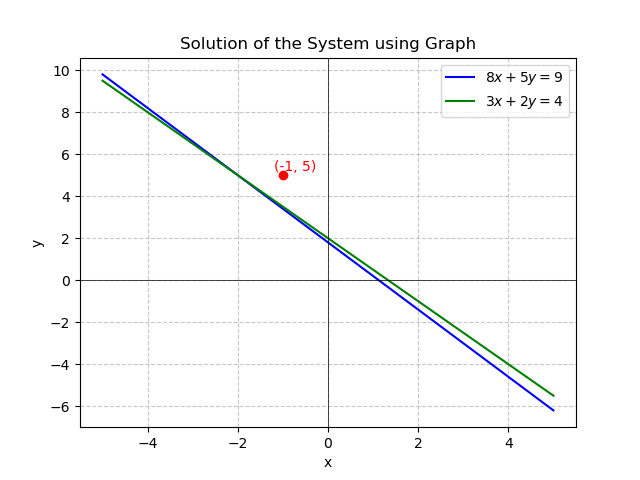
\includegraphics[width=\columnwidth, height=0.8\textheight, keepaspectratio]{Figs/Fig1.png}     
\end{frame}

\end{document}